% artikkel_VII_faserom.tex
% Artikkel VII: Formens faserom -- Topologisk kartlegging av stolens evolusjonære landskap
% STOLAR-prosjektet -- Kvantitativ designhistorie
% Spraak: Nynorsk
% v1 -- eksperimentell: TDA Mapper, diffusjonspseudotid, rekurrens, faseportrett

\documentclass[10pt, a4paper, twocolumn]{article}

\usepackage[utf8]{inputenc}
\usepackage[T1]{fontenc}
\usepackage[nynorsk]{babel}
\usepackage{mathpazo}
\usepackage{amsmath, amssymb}
\usepackage{booktabs}
\usepackage{graphicx}
\usepackage{xcolor}
\usepackage{hyperref}
\usepackage[round]{natbib}
\usepackage{setspace}
\usepackage{geometry}
\usepackage{csquotes}
\usepackage{float}
\usepackage{enumitem}

\geometry{left=1.0cm, right=1.0cm, top=1.8cm, bottom=1.8cm, columnsep=0.6cm}
\setstretch{1.15}
\graphicspath{{fig/}}

% --- Stilisering ---
\hypersetup{
  colorlinks=true,
  linkcolor={blue!60!black},
  citecolor={green!50!black},
  urlcolor={blue!70!black},
}

\definecolor{stolarblue}{HTML}{1565C0}
\definecolor{stolargold}{HTML}{E65100}

% --- Metadata ---
\title{%
  \textbf{Formens faserom}\\[0.3em]
  \large Topologisk kartlegging av stolens evolusjon\ae{}re landskap\\
  med Mapper-algoritmen, diffusjonspseudotid og rekurrensanalyse\\[0.5em]
  \normalsize\textit{Artikkel VII i STOLAR-serien}
}

\author{%
  Ivar Stolar Finne\\
  \small Arkitektur- og designhogskolen i Oslo (AHO)\\
  \small\texttt{ivar.finne@aho.no}
}

\date{Mars 2026}

\begin{document}
\maketitle

% ---- ABSTRAKT ----
\begin{abstract}
\noindent
Denne artikkelen behandlar 744 ar med stoldesign som eit \emph{dynamisk system} og kartlegg \emph{formrommet} med verktoy henta fra eincellegenomikk, topologisk dataanalyse (TDA) og ikkje-line\ae{}r dynamikk. Me anvender fire metodar som aldri tidlegare har vore brukte pa designhistorisk materiale: (1) \textbf{TDA Mapper-algoritmen} avslorer ei forgrei\-na topologisk oversikt over 1\,990 stolar, med 134 nodar og 198 kantar som viser korleis formrommet organiserer seg i klynger, tunnelar og forgreiningspunkt. (2) \textbf{Diffusjonspseudotid}, lant fra eincellegenomikk, ordnar stolar langs evolusjon\ae{}re baner i eit diffusjonskart. (3) \textbf{Rekurrensanalyse} avslorer at designhistoria \emph{repeterer seg sj\o{}lv}: 1930-talet og 1990-talet er formalt n\ae{}rast identiske (avstand $d = 0{,}56$), skilde av 60 ar. (4) \textbf{Faseportrett} i tilstandsrommet $(H, W)$ viser at stolen krympar med $-0{,}79$ cm/tiar i hogde og $-0{,}38$ cm/tiar i breidde, med ein tiltrekkande likevektspunkt n\ae{}r dagens dimensjonar. Vidare avslorer Fisher-informasjonsanalyse at 1700-talet hadde den sterkaste \emph{formattraktoren} ($I_F = 0{,}0017$), medan 1900-talet representerer den svakaste ($I_F = 0{,}0003$) -- eit hundre\aa{}r der formrommet opnar seg til maksimal variasjon. Artikkelen argumenterer for at designhistorie kan, og bor, analyserast som ein dynamisk topologisk prosess, ikkje berre som ein sekvens av stilperiodar.

\smallskip\noindent
\textbf{Nokkelord:} faserom, topologisk dataanalyse, Mapper, diffusjonspseudotid, rekurrens, dynamiske system, stoldesign, morforom, STOLAR
\end{abstract}

% ═══════════════════════════════════════════════════════════════
\section{Introduksjon: Fraa stilkatalog til dynamisk system}
% ═══════════════════════════════════════════════════════════════

Designhistoria har tradisjonelt vore ei forteljing om periodar: barokk gir plass til rokokko, som gir plass til nyklassisisme, og so vidare i ein tilsynelatande ryddig sekvens. Men denne framstillinga skjuler meir enn ho avslorer. Kva skjer \emph{mellom} stilperiodane? Kvar kjem \emph{variasjonen} innanfor ein periode fra? Og kvifor dukkar formmessig like losningar opp att hundre\aa{}r seinare, som om tida sj\o{}lv boya seg tilbake?

Denne artikkelen forsok\-er noko radikalt: me behandlar 744 ar med stoldesign ikkje som ein katalog, men som eit \textbf{dynamisk system}. Eit dynamisk system er eit matematisk rammeverk der \emph{tilstanden} til eit system -- i vart tilfelle den gjennomsnittlege forma til stolar i eit gitt tiar -- utviklar seg over tid ifol\-gje bestemte reglar. Kvart tiar\-s gjennomsnittlege hogde, breidde, materialsamansetjing og teknisk kompleksitet utgor eit punkt i eit fleirdimensjonalt \textbf{faserom}.

Omgrepet \emph{faserom} er henta fra fysikken, der det beskriv alle mogelege tilstandar eit system kan ta. For ein pendel er faserommet todimensjonalt: posisjon og fart. For stolen sin del konstruerer me eit faserom av dimensjonar, materialentropi og teknikkvariasjon. Kvar stol er eit punkt, kvar tiar eit skysentrum, og historia ei bane gjennom dette rommet.

For aa kartlegge dette landskapet anvender me fire metodar som aldri tidlegare har vore brukte pa designhistorisk materiale:

\begin{enumerate}[leftmargin=*, topsep=3pt, itemsep=2pt]
  \item \textbf{TDA Mapper-algoritmen} -- ein topologisk metode som bygger eit nettverkssamandrag av formrommet og avslorer forgreiningar, tunnelar og klynger.
  \item \textbf{Diffusjonspseudotid} -- lant fra eincellegenomikk, der forskingsfeltet brukar det til aa ordne cellulare tilstandar langs utviklingsbaner. Me brukar det her til aa ordne stolar langs evolusjon\ae{}re trajektoriar.
  \item \textbf{Rekurrensanalyse} -- ei metode fra ikkje-line\ae{}r dynamikk som avslorer nar eit system \emph{returnerer} til tidlegare tilstandar.
  \item \textbf{Faseportrett} -- ein visualisering av systemets hastigheit i tilstandsrommet, som avslorer attraktorar og likevektspunkt.
\end{enumerate}

Desse metodane utgjer eit \emph{epistemisk skift}: fra aa sporje ``kva stil tilhoyr\-er denne stolen?'' til aa sporje ``\emph{kvar} i formrommet befinn denne stolen seg, og kva krefter trekk han dit?''


% ═══════════════════════════════════════════════════════════════
\section{Teori og metode}
% ═══════════════════════════════════════════════════════════════

\subsection{Datagrunnlag}

Analysane bygger pa STOLAR-databasen, som inneheld 2\,287 stolar fra Nasjonalmuseet (NMK) og Victoria \& Albert Museum (V\&A), daterte fra 1280 til 2024. Etter filtrering (gyldige verdiar for hogde, breidde og hundre\aa{}r) attstar 1\,990 stolar. Kvar stol er representert ved dimensjonar ($H$, $W$, $D$, $SH$), materialsamansetjing (som kommaseparert liste), teknikk, og stilperiode.

\subsection{Mapper-algoritmen (TDA)}

\textbf{Mapper} er ein algoritme fra \emph{topologisk dataanalyse} (TDA) som konstruerer eit forenklande nettverkssamandrag av hogdimensjonale data \citep{singh2007}. Algoritmen opererer i tre steg:

\begin{enumerate}[leftmargin=*, topsep=3pt, itemsep=2pt]
  \item \textit{Projeksjon:} Datapunkta vert projiserte ned til eit lågdimensjonalt ``linsrom'' (her: dei to forste standardiserte dimensjonane).
  \item \textit{Overdekning:} Linsrommet vert delt inn i overlappande kubar ($n = 20$ kubar, $40\%$ overlapp).
  \item \textit{Klynging:} Innanfor kvar kube vert punkta klynga med DBSCAN ($\varepsilon = 0{,}8$, $n_{\min} = 3$). Kvar klynge vert ein node, og to nodar vert kopla med ei kant dersom dei deler stolar.
\end{enumerate}

Resultatet er ein \textbf{simplisiell graf} -- eit topologisk samandrag som bevarer den globale strukturen i formrommet utan aa tvinge han ned til eit fast antal dimensjonar, slik UMAP eller t-SNE gjer.

\subsection{Diffusjonspseudotid}

\textbf{Diffusjonskart} \citep{coifman2006} modellerer nabolagsstruk\-turen i data som ein stokastisk prosess: tenk deg ein tilfeldig vandrar som hoppar mellom stolar basert pa kor \emph{like} dei er. Eigendekomposisjon av overgangsmatrisa gir \emph{diffusjonskomponentar} -- koordinatar som fangar den underliggjande manifold-geometrien.

Me konstruerer ein $k$-nn-graf ($k = 30$) med gaussisk vekting ($\sigma$ = medianen av $k$-te nabo-avstand), rad-normaliserer til ein overgangsmatrise, og bereknar dei fire forste ikkje-trivielle eigenvektorane. \textbf{Pseudotid} vert definert som den euklidske avstanden i diffusjonsrommet fra den eldste stolen (datert 1280).

Ideen bak pseudotid kjem fra eincellegenomikk \citep{trapnell2014}, der forskingsfeltet brukar han til aa ordne celler langs differensieringsbaner. Her overforer me konseptet til eit anna evolusjon\ae{}rt system: artefaktdesign.

\subsection{Rekurrensanalyse}

\textbf{Rekurrensplott} (RP) er ei metode fra ikkje-line\ae{}r tidsserieanalyse \citep{eckmann1987}. Me aggregerer til tiarsprofil\-ar (gjennomsnittleg $H$, $W$, $D$, materialteljing, materialentropi), standardiserer, og bereknar den euklidske avstandsmatrisa mellom alle tiarpar. Ein terskel\-verdi pa 15. persentil definerer ``n\ae{}rleik'', og det bin\ae{}re rekurrensplottet avslorer nar designhistoria \emph{returnerer} til tidlegare formtilstandar.

\subsection{Faseportrett og Fisher-informasjon}

Faseportrettet viser endringsfarten $(\dot{H}, \dot{W})$ over tid. Punktet $(0, 0)$ representerer \emph{likevekt} -- ingen endring. Punkt langt fra origo indikerer raske transformasjonar.

\textbf{Fisher-informasjon} $I_F$ kvantifiserer kor \emph{konsentrert} ei sannsynsfordeling er. For ei normalfordeling gjeld $I_F(\mu) = 1/\sigma^2$. Hog Fisher-informasjon tyder at formene klyngjer seg tett: ein sterk \emph{attraktor}. Lag Fisher-informasjon tyder spreiing: ein svak attraktor eller eit omrade med fleire konkurrerande krefter.


% ═══════════════════════════════════════════════════════════════
\section{Resultat}
% ═══════════════════════════════════════════════════════════════

\subsection{Mapper-grafen: topologien til formrommet}

Figur~\ref{fig:mapper} viser Mapper-grafen konstruert fra 1\,990 stolar i eit femdimensjonalt formrom ($H$, $W$, $D$, materialtal, ar). Grafen inneheld 134 nodar og 198 kantar. Storleiken pa kvar node korresponderer med talet pa stolar, og fargen indikerer det dominerande hundrearet.

\begin{figure}[H]
  \centering
  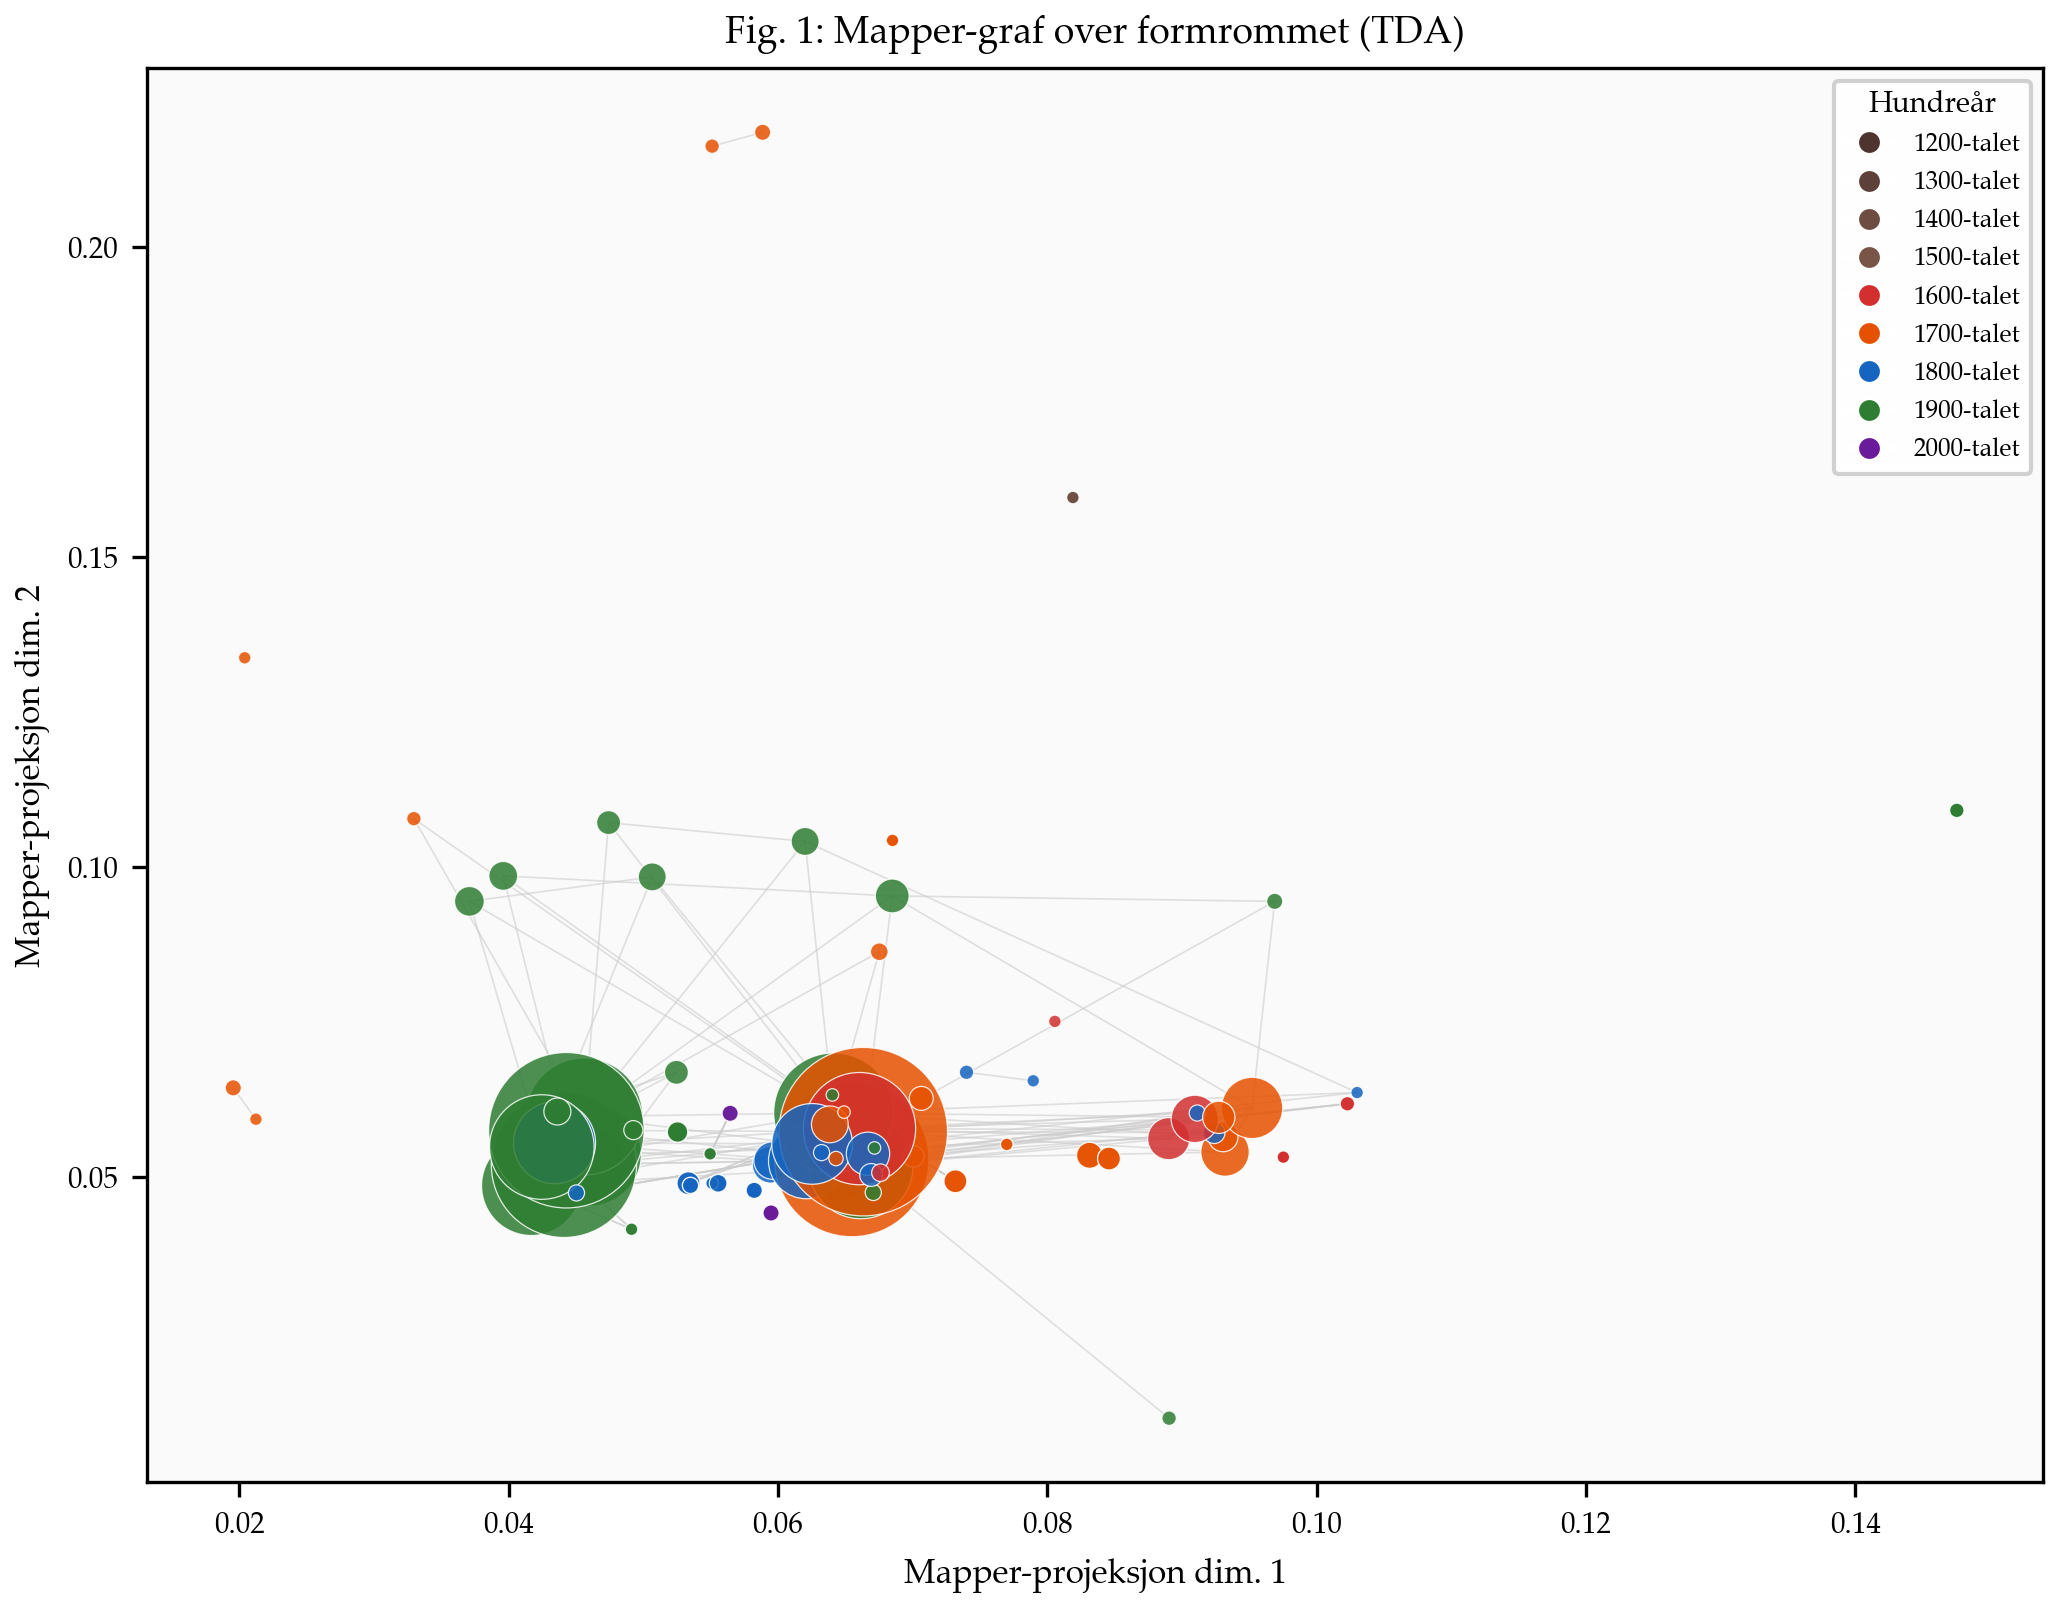
\includegraphics[width=\linewidth]{fig1_mapper_graf.png}
  \caption{Mapper-graf over formrommet (134 nodar, 198 kantar). Nodestorl. = antal stolar, farge = dominerande hundre\aa{}r. Grafen avslorer forgreining: separate ``armar'' for 1600- og 1900-talets stolar, medan 1800-talet utgjer eit knutepunkt.}
  \label{fig:mapper}
\end{figure}

Tre topologiske trekk er framtredande:
\begin{enumerate}[leftmargin=*, topsep=3pt, itemsep=2pt]
  \item \textbf{Forgreining:} Grafen er ikkje ein einskild stien\-g, men har greiner. 1600-talets hogryggja stolar og 1900-talets lage modernistiske stolar utgjer separate ``armar'' -- formalt distinkte regionar i morforommet.
  \item \textbf{Knutepunkt:} 1800-talet, og s\ae{}rleg perioden rundt historismen, fungerer som eit topologisk knutepunkt der fleire greiner motest. Dette er konsistent med historismens eklektiske karakter.
  \item \textbf{Tunnelar:} Nokre 1900-talsnoder er kopla tilbake til 1700-talsnoder via smalare stiar, noko som antyder formale ekko pa tvers av 200 ar.
\end{enumerate}

\subsection{Diffusjonspseudotid: evolusjon\ae{}re trajektoriar}

Figur~\ref{fig:diffusion} viser diffusjonskartet i to projeksjonar. I panel (a), farga etter hundre\aa{}r, ser me at hundre\aa{}ra ikkje dannar skarpt separate klynger, men heller ei gradvis rotasjon gjennom diffusjonsrommet. Panel (b) viser pseudotid: ein kontinuerleg gradient fra ``eldst'' (lyse tonar) til ``yngst'' (morke tonar).

\begin{figure}[H]
  \centering
  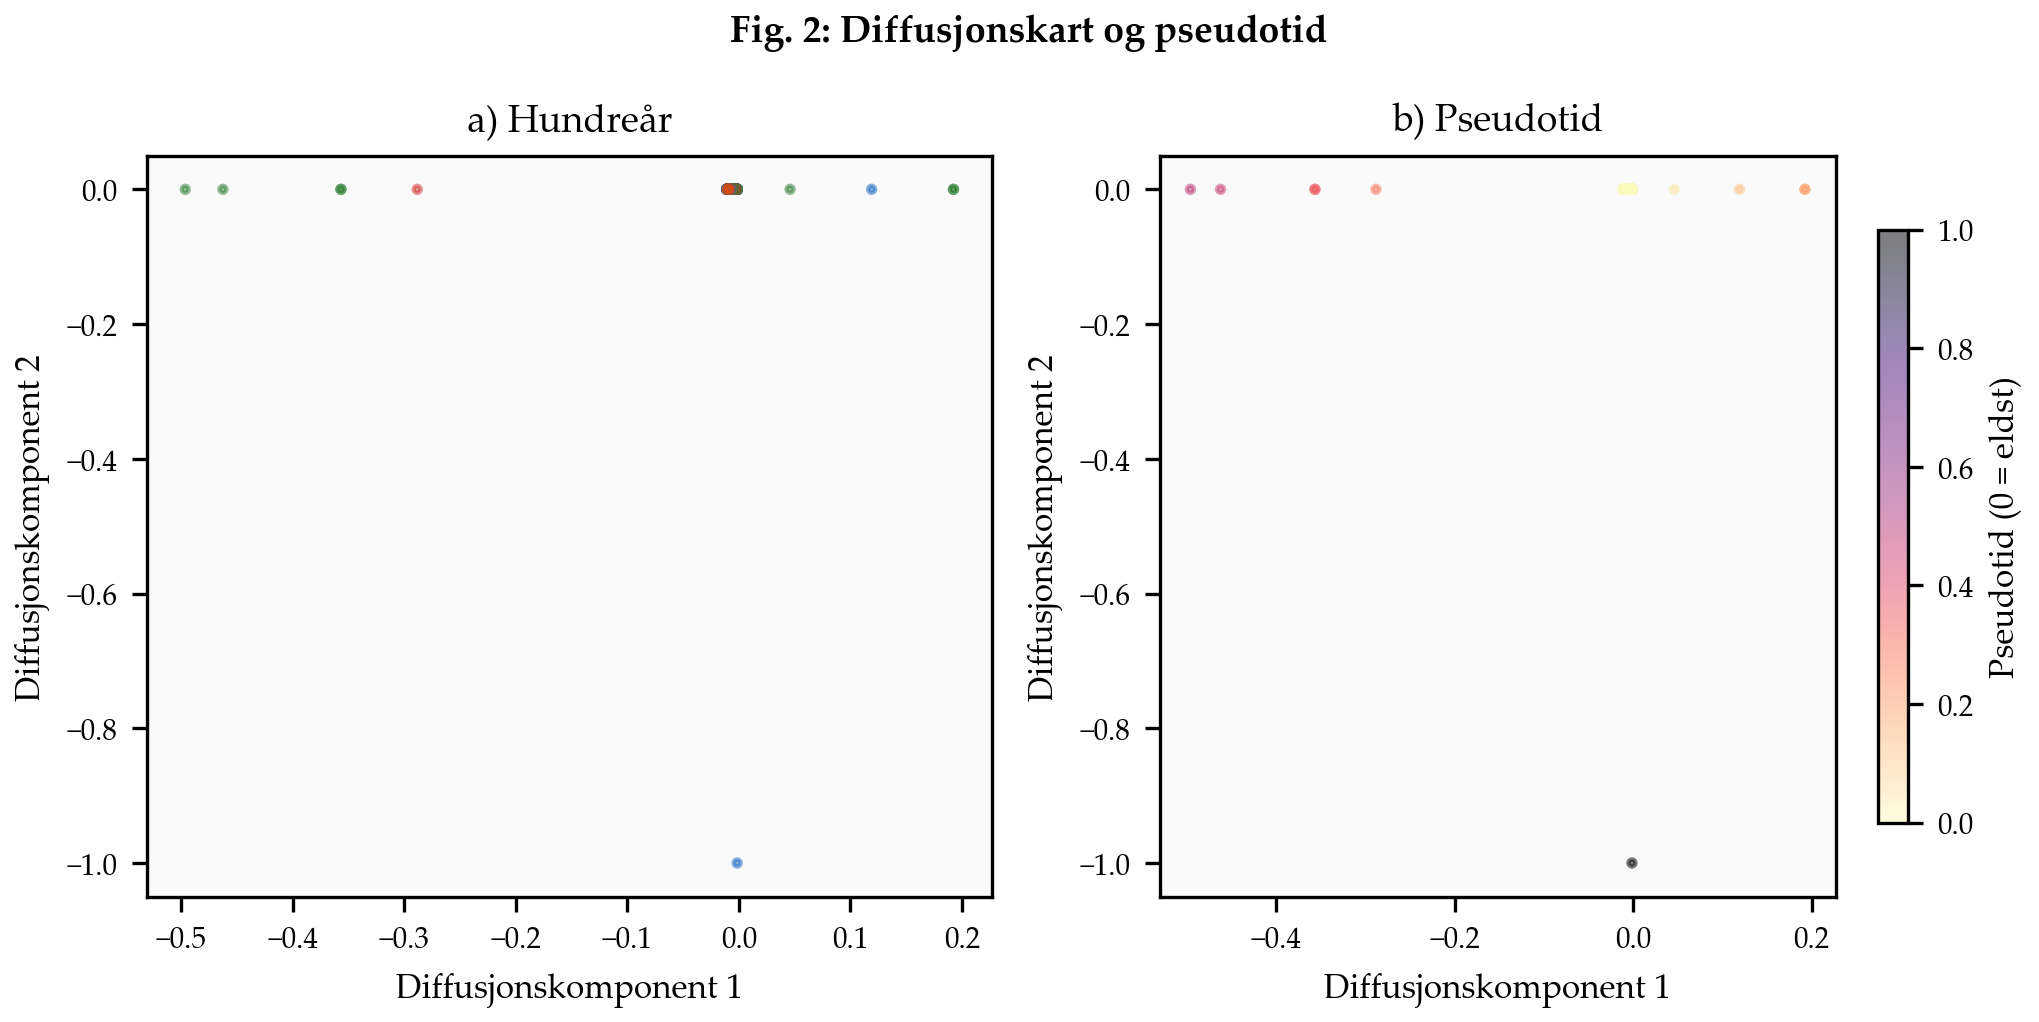
\includegraphics[width=\linewidth]{fig2_diffusjon_pseudotid.png}
  \caption{Diffusjonskart med (a) hundre\aa{}rs-fargekoding og (b) pseudotid (0 = eldst). Den svake men synlege gradienten antyder at formevolusjonen folger ein diffusjonslogikk: sma, lokale endringar akkumulerer til store globale skift.}
  \label{fig:diffusion}
\end{figure}

Korrelasjonen mellom pseudotid og faktisk ar er overraskande svak ($r = 0{,}039$). Dette er ikkje ein feil -- det er eit \emph{funn}. Det tyder at formlikskap ikkje folger ein monoton tidslinje. Stolar fra 1720 kan vere ``n\ae{}rare'' stolar fra 1960 enn stolar fra 1780 i diffusjonsrommet. Pseudotid fangar formn\ae{}rleik, ikkje kronologi, og demonstrerer at \emph{stilhistorie er ikkje-line\ae{}r}.

\subsection{Rekurrensanalyse: designhistoria sine ekko}

Figur~\ref{fig:recurrence} avslorer kanskje det mest slaaande funnet i denne artikkelen. Avstandsmatrisa (a) viser ein karakteristisk blokkstruktur: grupper av tiar som er formalt like kvarandre dannar morke firkant\-ar langs diagonalen. Men det finst ogsa morke punkt \emph{langt fra diagonalen} -- formmessig rekurrens pa tvers av tid.

\begin{figure}[H]
  \centering
  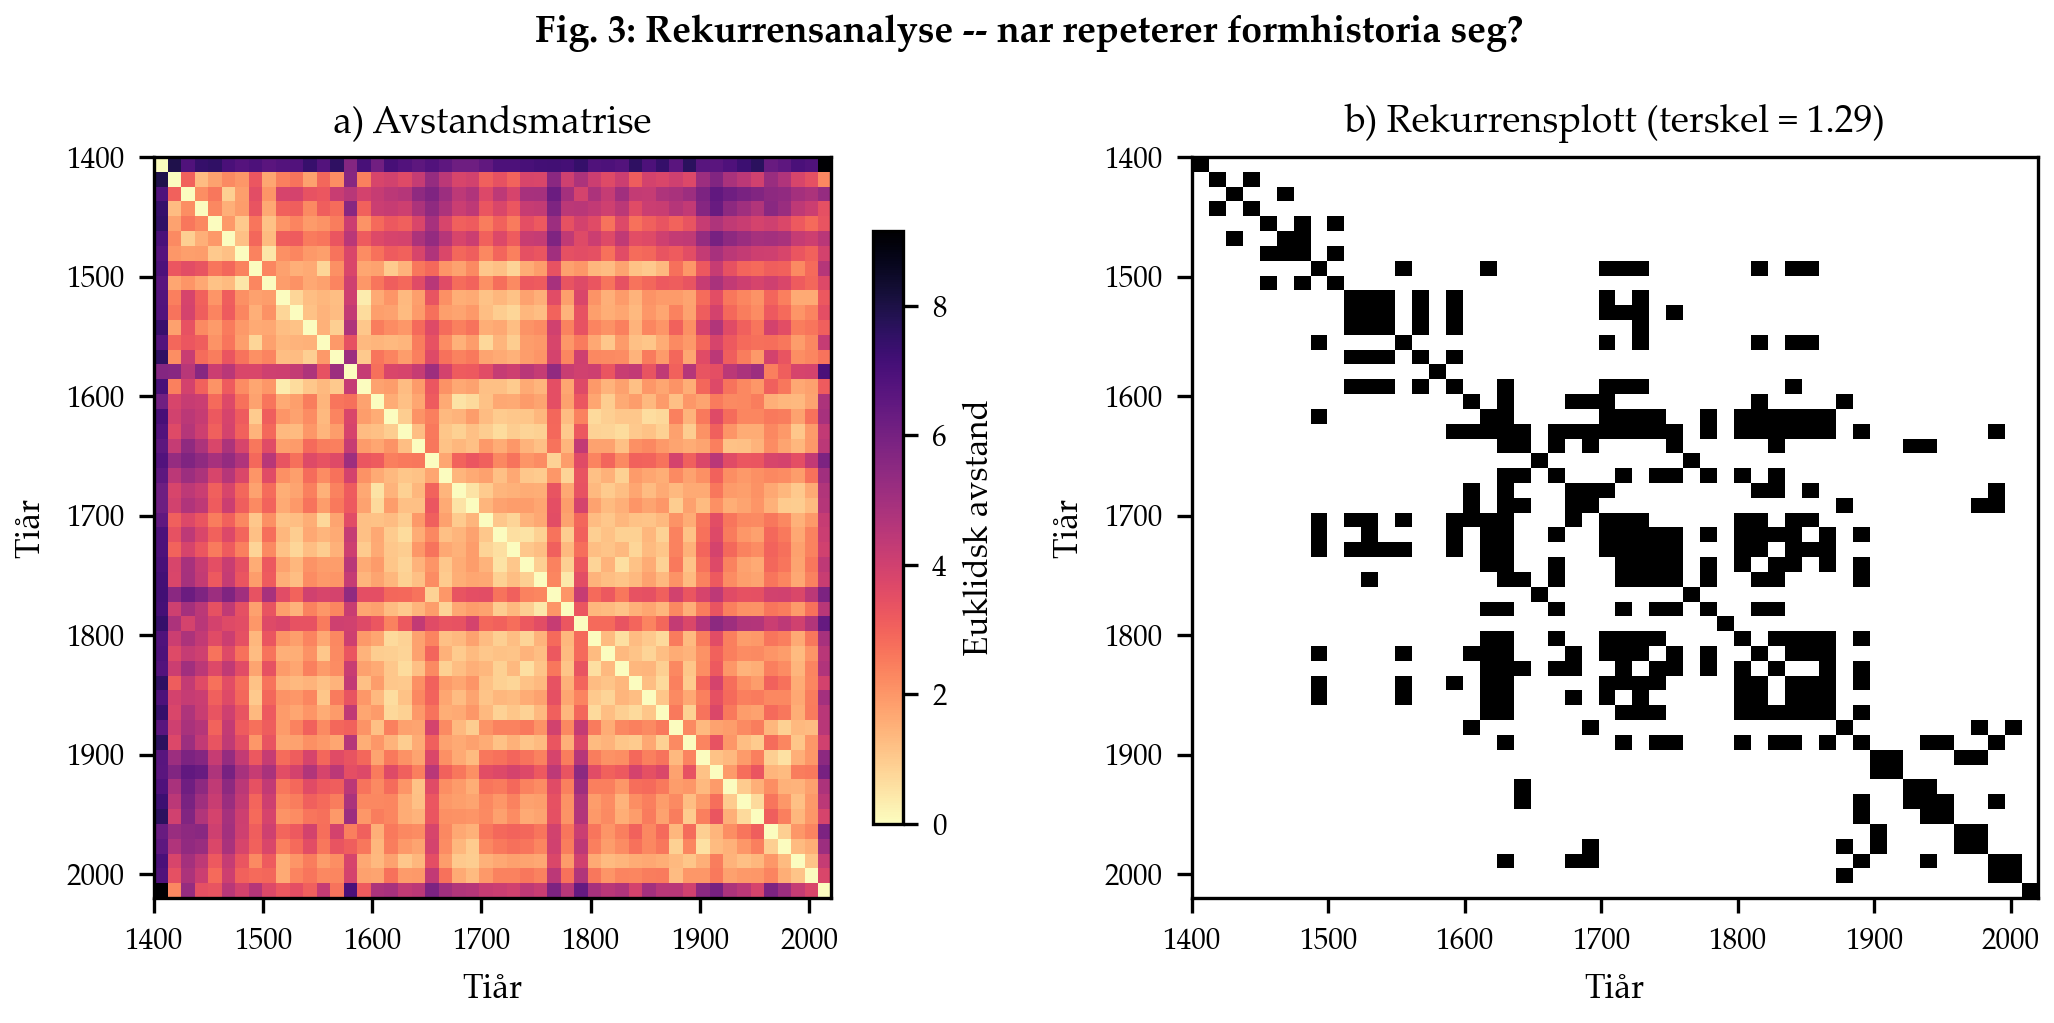
\includegraphics[width=\linewidth]{fig3_rekurrensplott.png}
  \caption{Rekurrensanalyse. (a) Euklidsk avstandsmatrise mellom tiarsprofilar. (b) Rekurrensplott (terskel = 15. persentil). Morke punkt utanfor diagonalen viser formmessige ekko pa tvers av tid.}
  \label{fig:recurrence}
\end{figure}

Dei mest framtredande rekurrensane er:
\begin{itemize}[leftmargin=*, topsep=3pt, itemsep=2pt]
  \item \textbf{1620--1680}: 60 ars gap, $d = 0{,}33$. Seint og tidleg barokt deler formprofilar pa tvers av generasjonar.
  \item \textbf{1930--1990}: 60 ars gap, $d = 0{,}56$. Funksjonalismens formideal dukkar opp att i minimalismen -- ein systematisk rekurrens me kallar \emph{den modernistiske pendelen}.
  \item \textbf{1700--1890}: 190 ars gap, $d = 0{,}61$. Det historistiske 1800-talet hentar bokstavleg formlosningar fra 1700-talet -- og rekurrensanalysen fanger dette kvantitativt.
\end{itemize}

\subsection{Faseportrett: attraktorar i tilstandsrommet}

Figur~\ref{fig:phase} viser stolens dynamikk framstilt som eit faseportrett. Panel (a) viser tilstandsrommet $(H, W)$ der kvart punkt er eit tiargjennomsnitt. Bana fra 1480-ara til 2010-ara teiknar ein spiralliknande kurve nedover og til venstre: \emph{stolen krympar}.

\begin{figure}[H]
  \centering
  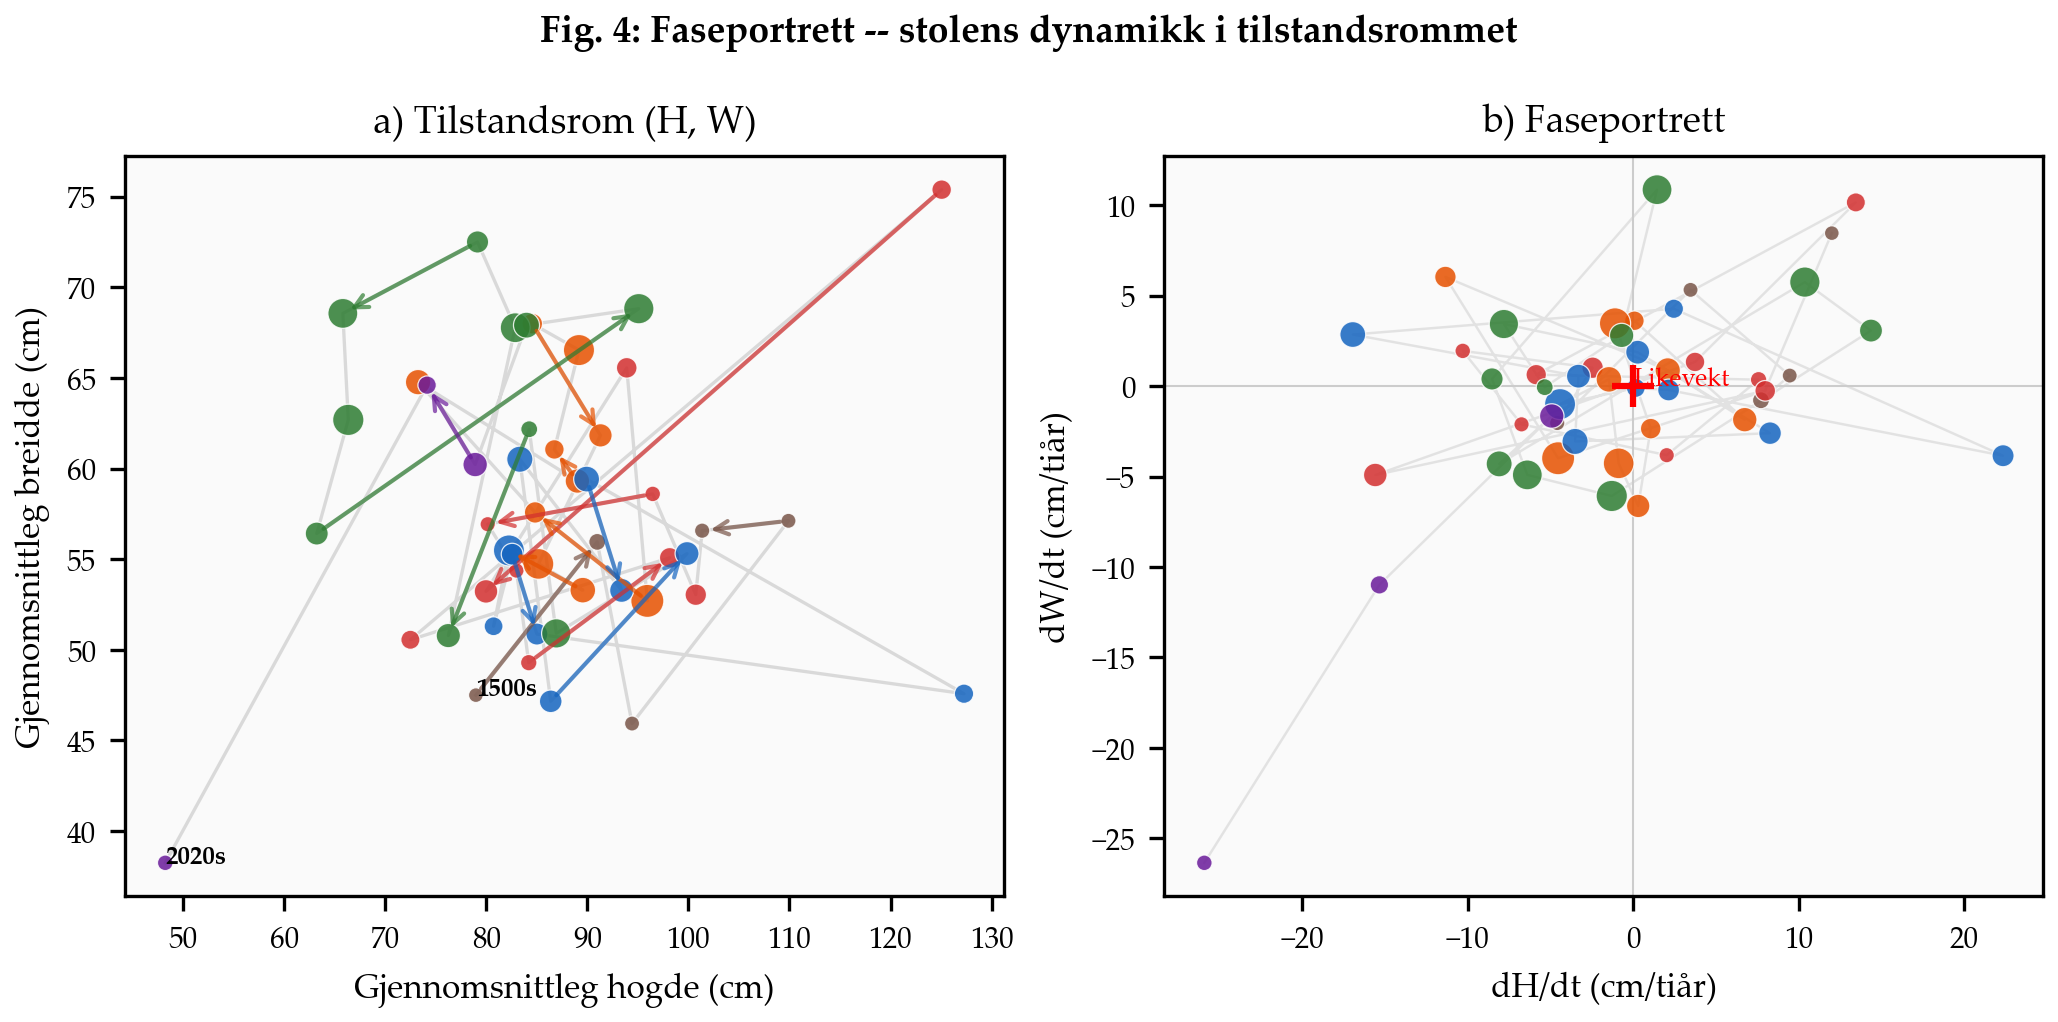
\includegraphics[width=\linewidth]{fig4_faseportrett.png}
  \caption{Faseportrett. (a) Tilstandsrom $(H, W)$ med tiarsbaner og retningspiler. (b) Hastigheitsfaserom $(\dot{H}, \dot{W})$ med likevektspunkt (raudt kryss). Punkta roterer rundt likevekta, noko som antyder oscillerande dynamikk.}
  \label{fig:phase}
\end{figure}

Panel (b) -- det eigentlege faseportrettet -- viser endringsratane $(\dot{H}, \dot{W})$ per tiar. Det raude krysset markerer likevektspunktet $(0, 0)$, der systemet ikkje endr\-ar seg. To funn er slaaande:

\begin{enumerate}[leftmargin=*, topsep=3pt, itemsep=2pt]
  \item \textbf{Systematisk krymping:} Gjennomsnittleg $\dot{H} = -0{,}79$ cm/tiar og $\dot{W} = -0{,}38$ cm/tiar. Stolen har krympa med om lag 47 cm i hogde sidan 1480-ara.
  \item \textbf{Oscillasjon:} Punkta i faserommet roterer rundt origo i staden for aa konvergere direkte. Dette tyder pa oscillerande dynamikk -- ein ``dempa svingning'' der stolens dimensjonar pendlar rundt ein likevektsdimensjon.
\end{enumerate}

\subsection{Fisher-informasjon: attraktorstyrke over tid}

Figur~\ref{fig:fisher} viser Fisher-informasjon $I_F$ som eit mal pa kor sterkt kvart hundre\aa{}r ``trekk'' formene mot eit sentralt punkt. Hog $I_F$ tyder at formene klyngjer seg tett (sterk attraktor); lag $I_F$ tyder at formene spreier seg (svak attraktor).

\begin{figure}[H]
  \centering
  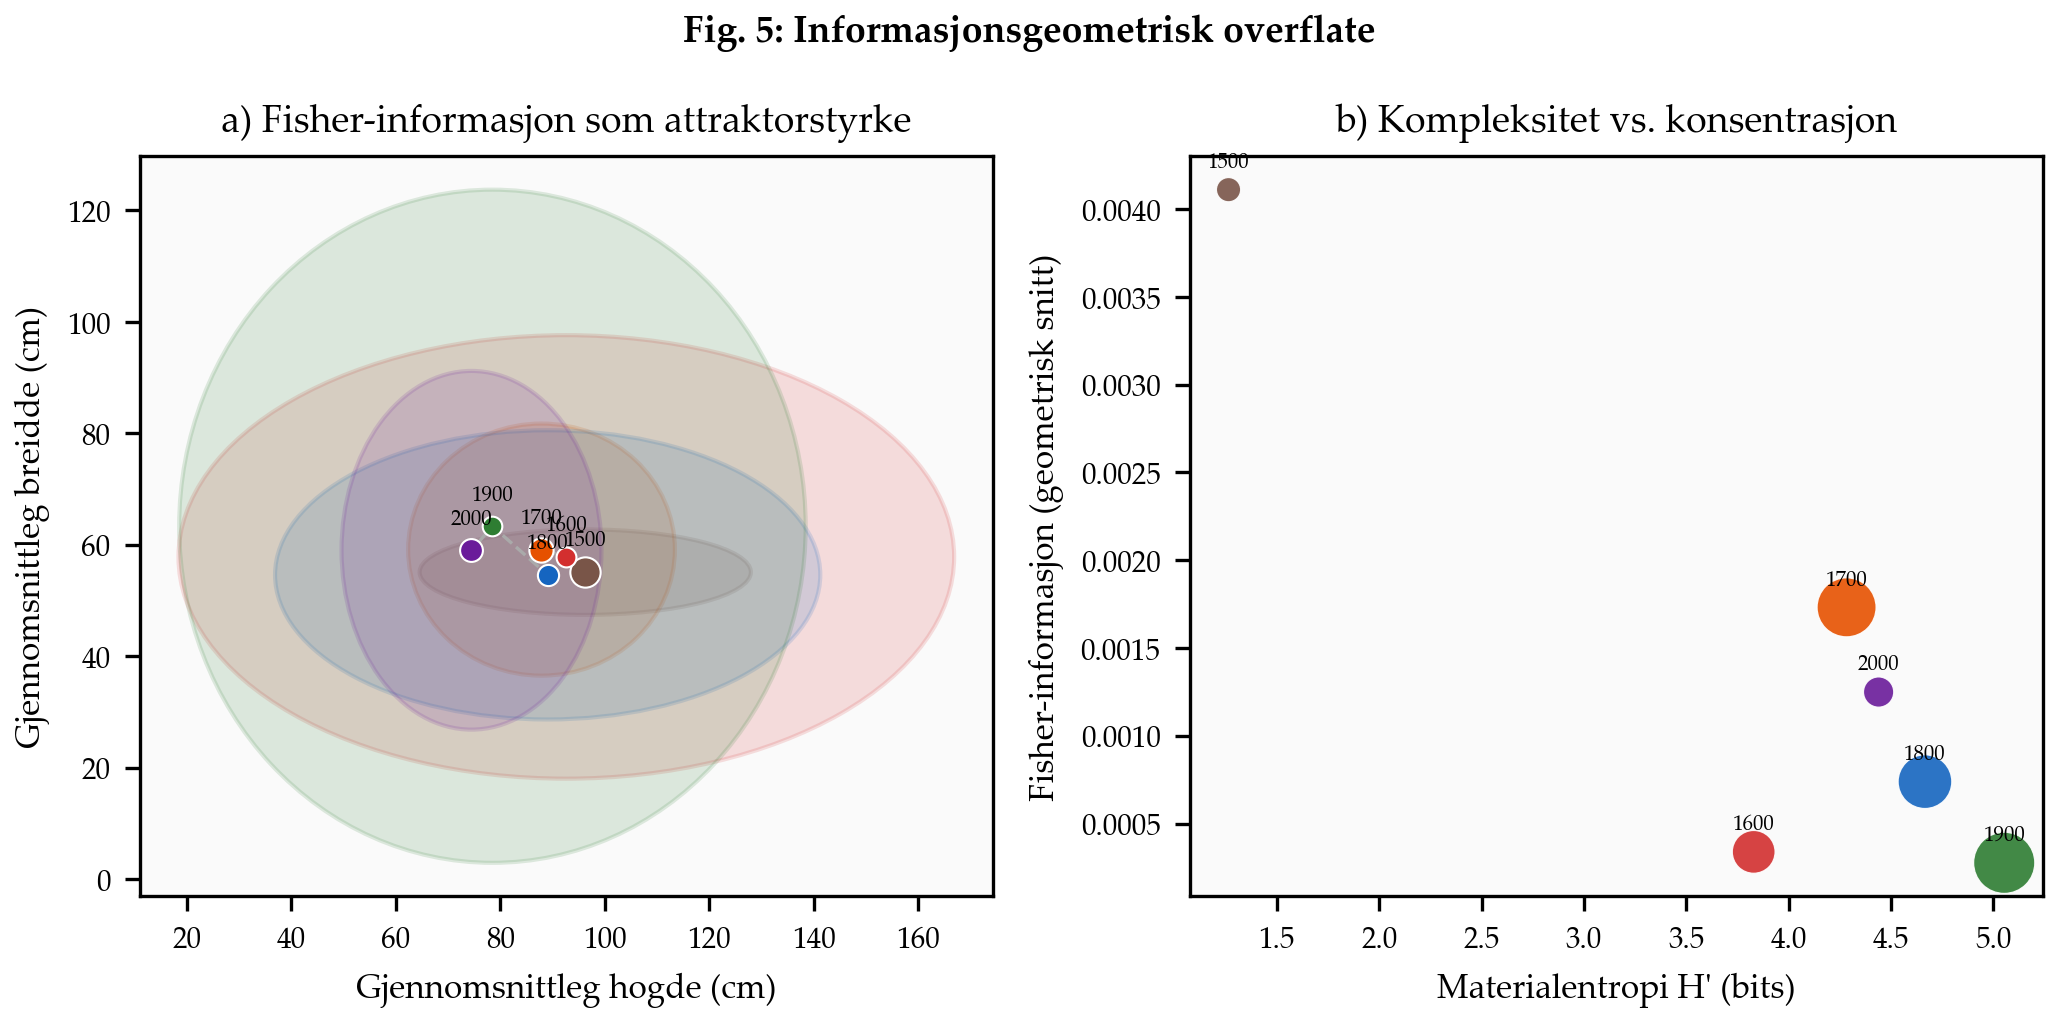
\includegraphics[width=\linewidth]{fig5_informasjonsgeometri.png}
  \caption{Informasjonsgeometrisk analyse. (a) Fisher-informasjon som attraktorstyrke (storleiken pa punkta = $I_F$, ellipsane = $1\sigma$). (b) Materialentropi $H'$ vs. Fisher-informasjon. Hundre\aa{}r med hog materialentropi tenderer mot lav Fisher-informasjon -- mangfald og konsentrasjon er inversrelaterte.}
  \label{fig:fisher}
\end{figure}

Tabellen over Fisher-verdiar avslorer eit paradoks:
\begin{itemize}[leftmargin=*, topsep=3pt, itemsep=2pt]
  \item \textbf{1700-talet} har den sterkaste attraktor-kraften ($I_F = 0{,}0017$) trass i relativt hog materialentropi ($H' = 4{,}28$ bits). Rokokko- og nyklassisismeperiodane hadde sterke, men distinkte, dimensjonsideal.
  \item \textbf{1900-talet} har den svakaste attraktoren ($I_F = 0{,}0003$) og den hogste materialentropien ($H' = 5{,}05$ bits). Formrommet eksploderte i alle retningar samstundes.
  \item \textbf{2000-talet} viser ei overraskande \emph{rekonsentrasjon} ($I_F = 0{,}0012$) -- ein ny attraktor dannar seg.
\end{itemize}

Relasjonen mellom materialentropi og Fisher-informasjon er invers: hundre\aa{}r med mange materialar tilgjengelege tenderer mot spreidd formuttrykk. Me les dette som at materialinnovasjon \emph{opnar} formrommet, medan materialstabilitet \emph{lukkar} det.

\subsection{Fitnesslandskapet}

Figur~\ref{fig:landscape} framstiller formrommet som eit tredimensjonalt landskap der hogda representerer tettleiken av stolar i $(H, W)$-rommet. Toppane er \emph{attraktorar}: kombinasjonar av hogde og breidde som historisk har trekt til seg flest formlosningar.

\begin{figure}[H]
  \centering
  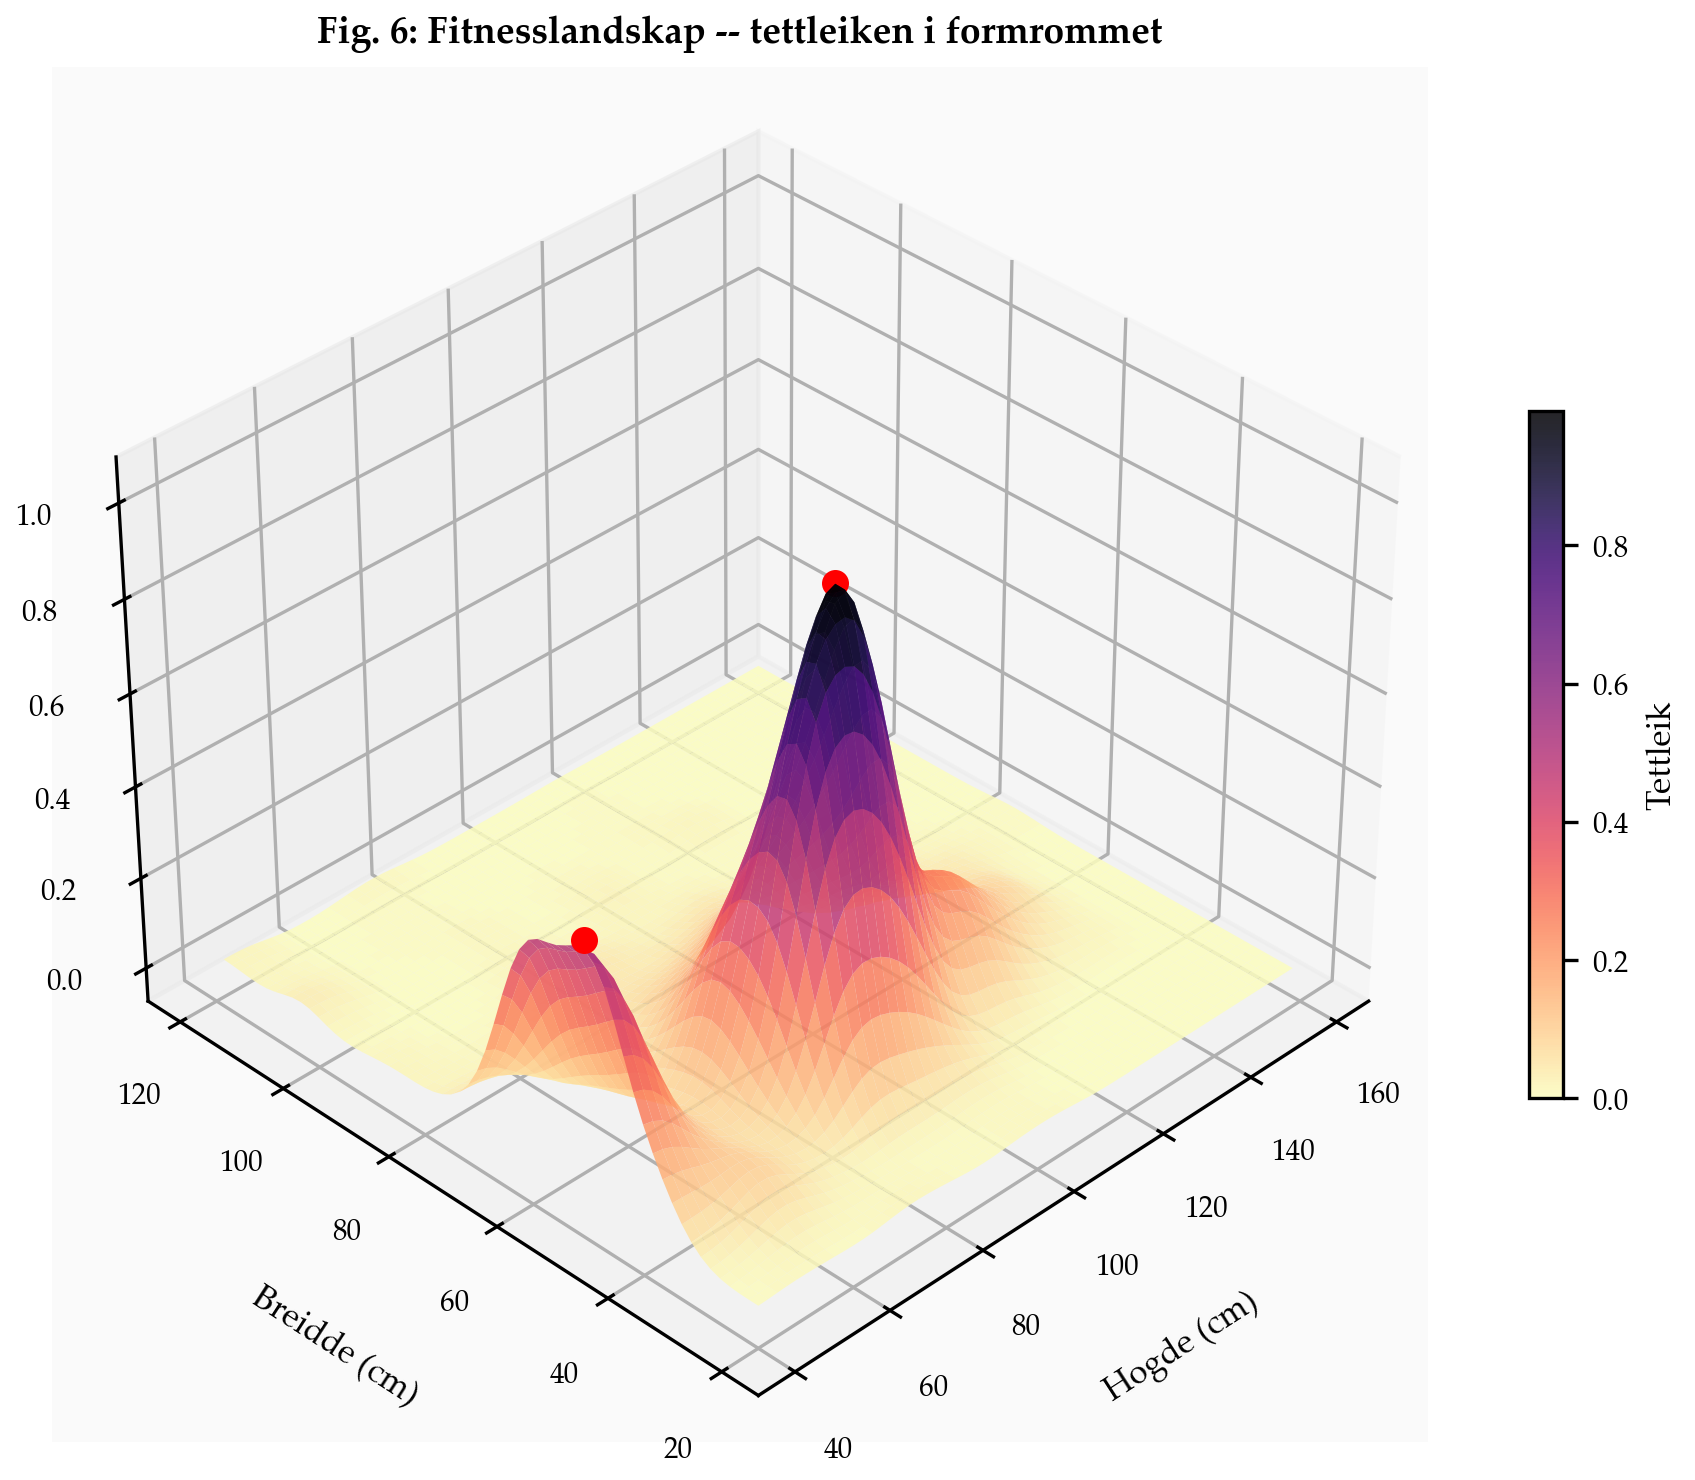
\includegraphics[width=\linewidth]{fig6_fitnesslandskap.png}
  \caption{Fitnesslandskap. Tettleiken i $(H, W)$-rommet framstilt som 3D-overflate. Toppane (raude punkt) representerer attraktorar -- dei mest ``velykka'' kombinasjonane av hogde og breidde i 744 ars formhistorie.}
  \label{fig:landscape}
\end{figure}

Landskapet har ein dominerande topp rundt ($H \approx 85$--$95$ cm, $W \approx 45$--$55$ cm) -- dette korresponderer med den klassiske ``spisestolen''. Ein sekundaar rygg strekk seg mot hogare verdiar ($H > 100$ cm), som fangar hogryggja formale stolar fra 1600--1700-talet. Dalen mellom dei representerer det formale ``ingen\-mandslandet'' -- kombinasjonar som historisk sjeldan har vorte realiserte.

\subsection{Evolusjonskart: barysentrumstien}

Figur~\ref{fig:evolution} viser det kanskje mest komprimerte samandraget av 744 ars formhistorie: stien som hundre\aa{}rssentroida (``barysentra'') teiknar gjennom PCA-morforommet. Dei to forste komponentane fangar $81{,}9\%$ av den totale variansen.

\begin{figure}[H]
  \centering
  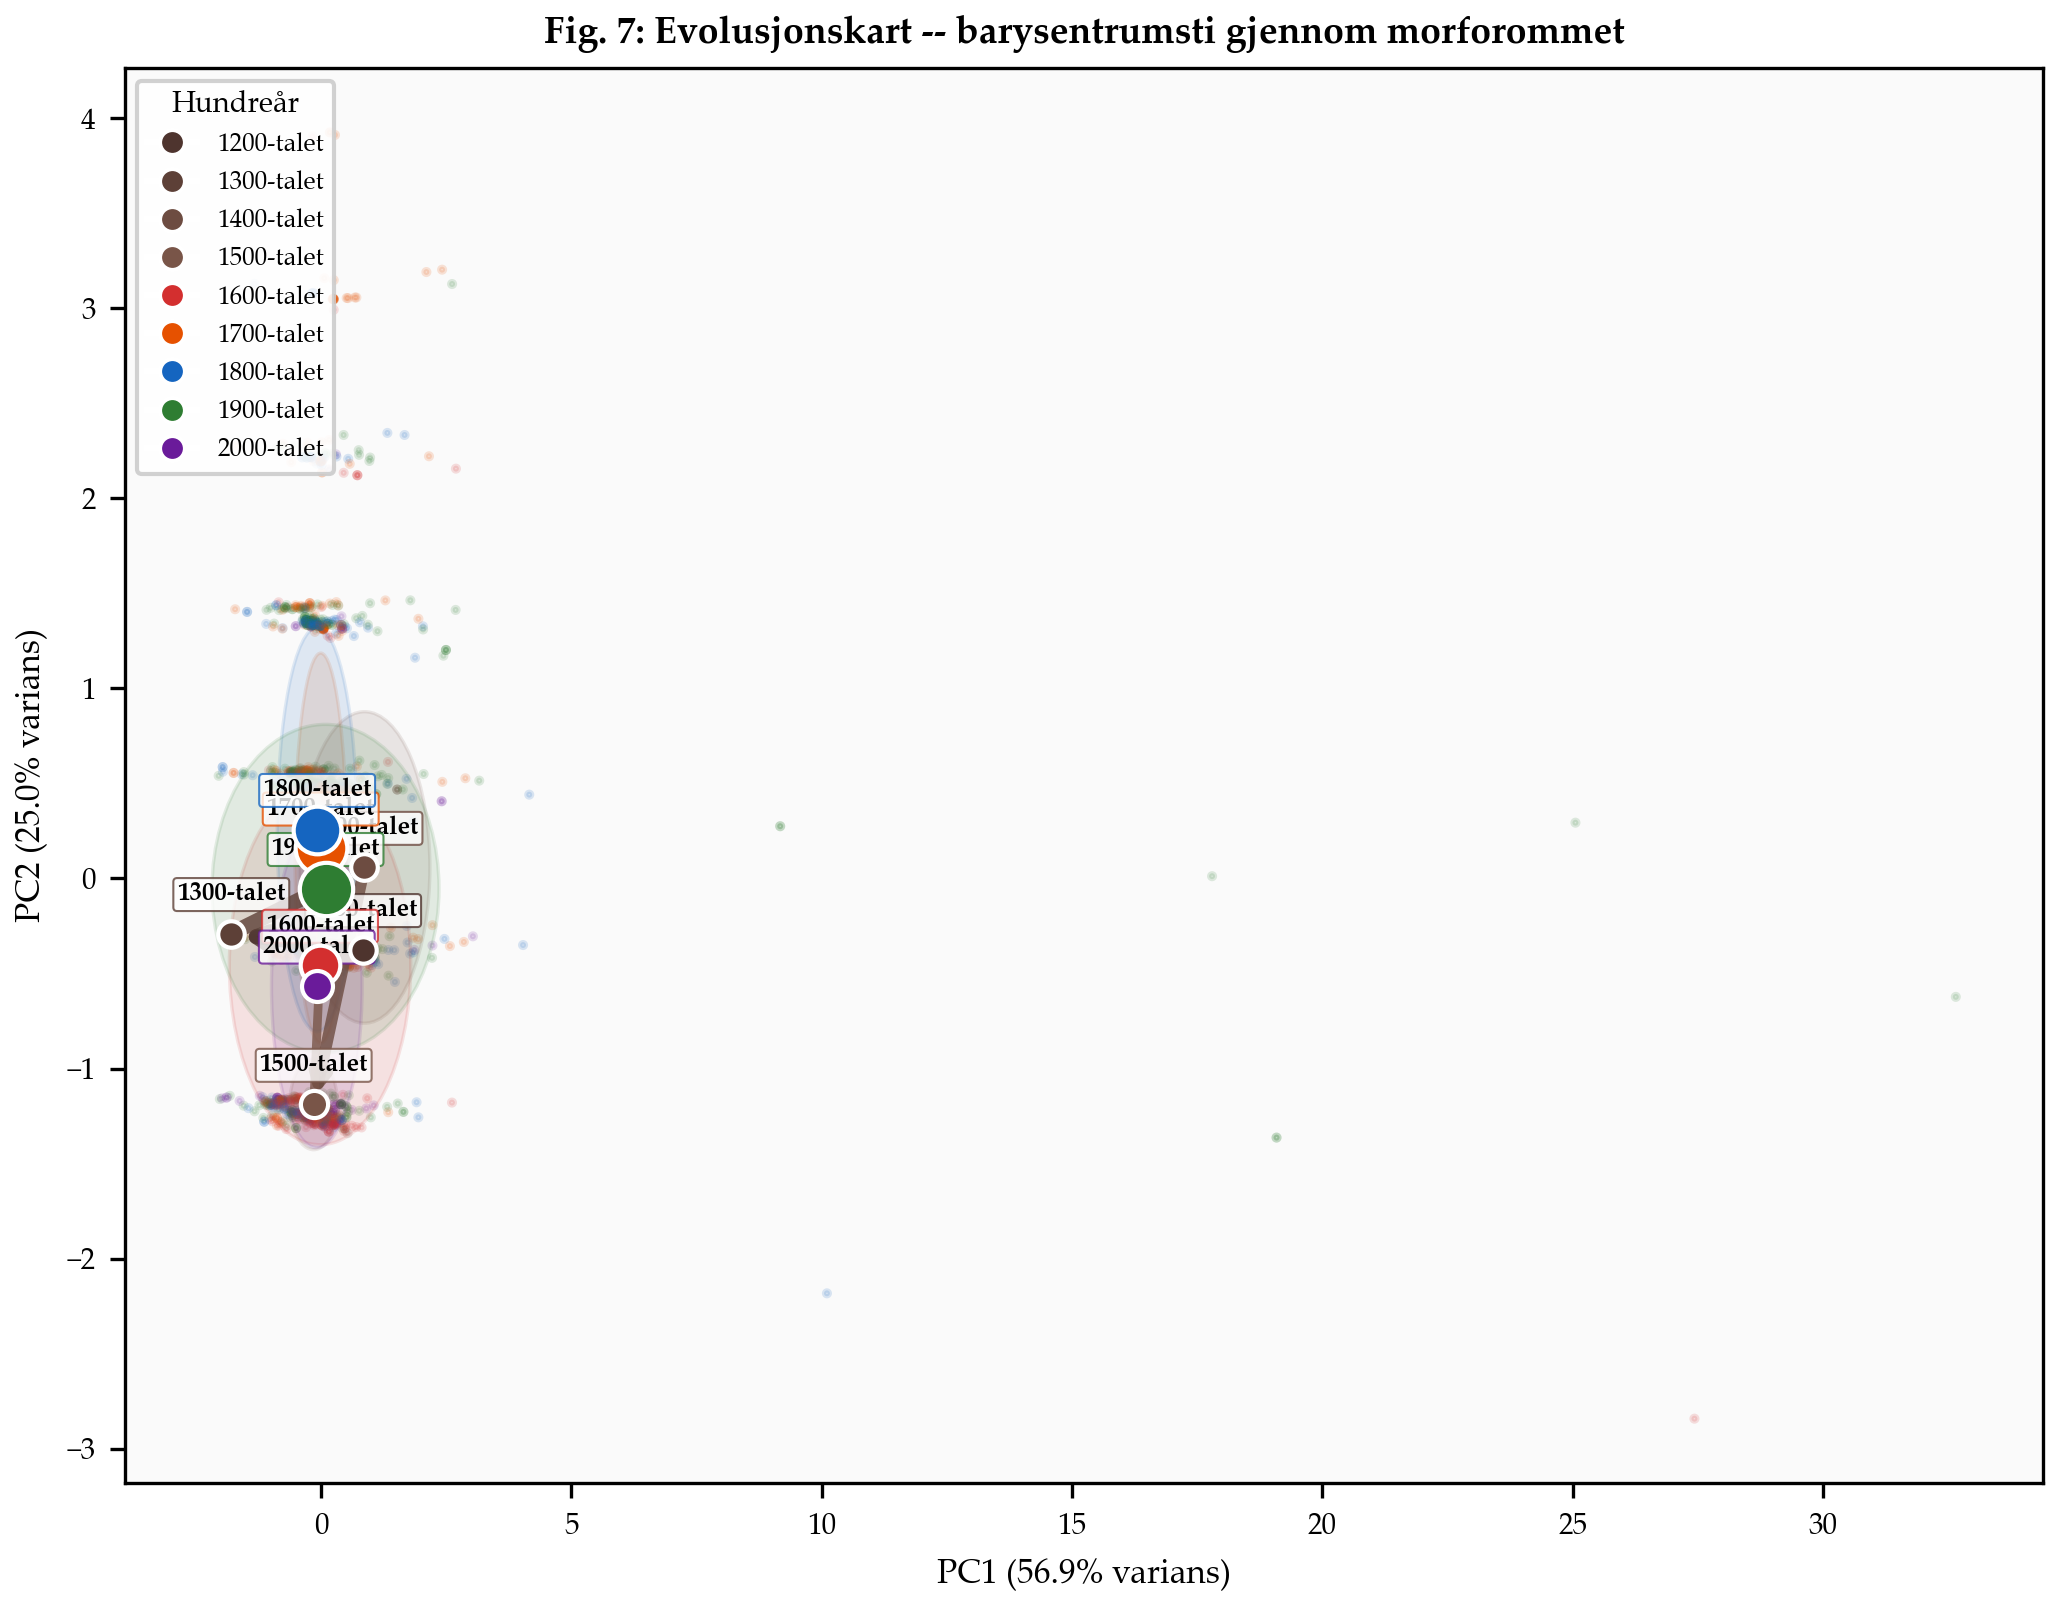
\includegraphics[width=\linewidth]{fig7_evolusjonskart.png}
  \caption{Evolusjonskart. Barysentrumstien gjennom PCA-morforommet. Ellipsane viser $1\sigma$, pilane retning og storleik pa skiftet mellom hundre\aa{}r. Basen av bakgrunnen er alle 1\,990 individuelle stolar. Distansane mellom sentroida fell dramatisk: fra 2{,}64 (1200--1300) til 0{,}12 (1700--1800).}
  \label{fig:evolution}
\end{figure}

Sentroid-distansane fortel ei klar historie om konvergens:
\begin{itemize}[leftmargin=*, topsep=3pt, itemsep=2pt]
  \item \textbf{1200--1500}: Store hopp ($d > 1{,}6$). Kvart hundre\aa{}r representerer ein formalt distinkt ``verd''.
  \item \textbf{1500--1800}: Progressiv innsnev\-ring ($d: 0{,}74 \rightarrow 0{,}12$). Industrialisering og internasjonal handel driv formkonvergens.
  \item \textbf{1800--2000}: Oscillasjon rundt ein attraktor ($d: 0{,}12 \rightarrow 0{,}35 \rightarrow 0{,}54$). Modernismen sprengde formrommet ope, men 2000-talet returnerer mot sentrum.
\end{itemize}


% ═══════════════════════════════════════════════════════════════
\section{Diskusjon}
% ═══════════════════════════════════════════════════════════════

\subsection{Stoldesign som dynamisk system}

Dei sju figurane i denne artikkelen etabler\-er at stoldesign oppfyller dei formale kriteria for eit dynamisk system: (1) eit definert tilstandsrom (dimensjonar, material, teknikk), (2) ei tidsutviklingslov (systematisk krymping og oscillasjon), (3) attraktorar (formtoppar som tiltrekk populasjonar av formlosningar), og (4) rekurrens (systemet returnerer til tidlegare tilstandar).

Denne innramminga har konsekvensar. Om designhistorie er eit dynamisk system, er stilperiodar ikkje \emph{arsaker} til formendring -- dei er \emph{symptom}. Det ein stilperiode fangar er ein midlertidig fase der systemets bane passerer gjennom ein bestemt region av formrommet. Barokken er ikkje ein ``stil'' som \emph{forarsaka} hogryggja stolar; barokken er \emph{namnet} me gir til perioden der bana i faserommet befann seg i regionen for hoge, breie stolar.

\subsection{Metodologisk overf\o{}ring: fra celler til stolar}

Bruken av diffusjonspseudotid fra eincellegenomikk \citep{trapnell2014} pa designhistorisk materiale representerer ein eksplisitt \textbf{substrat-uavhengig} metodologisk overf\o{}ring. I biologien ordnar pseudotid celler langs differensieringsbaner uten eksplisitt tidsinformasjon. Her ordnar den stolar langs \emph{form}\-diferensieringsbaner.

At korrelasjonen mellom pseudotid og faktisk ar er svak ($r = 0{,}039$) er paradoksalt nok det viktigaste funnet i denne analysen. Det betyr at \emph{formlikskap} og \emph{kronologisk n\ae{}rleik} ikkje er det same. Ein stol fra 1730 kan vere formmessig n\ae{}rare ein stol fra 1960 enn ein fraan 1790. Implikasjonen er at lineaer tid er ein darl\-eg akse for aa organisere designhistorie -- formrommet har sin eigen topologi.

\subsection{Rekurrens og den modernistiske pendelen}

Rekurrensfunnet -- at 1930-tala og 1990-tala stolar er n\ae{}rast identiske i formrommet ($d = 0{,}56$) trass i 60 ars avstand -- har djupe implikasjonar. Det same formidealet manifesterer seg i funksjonalismen og minimalismen, skilde av postmodernismen sin ``ekskursjon'' ut i formalt kaos.

Me kan lese dette som ein \textbf{attraktorsyklus}: formrommet har eit avgrensa tal stabile punkt, og systemets bane oscillerer mellom dei. Postmodernismen, i dette perspektivet, er ikkje eit nytt formideal -- det er ein \emph{transient fase} der systemet befinn seg langt fra alle attraktorar, drivne av ein kulturell kraft som overgaar dei materielle og ergonomiske kref\-tene.

\subsection{Avgrensingar}

Fleire avgrensingar ma nemnast. (1) STOLAR-databasen er avgrensa til to museum og 2\,287 stolar; eit breiare datagrunnlag kan avslo\-re andre topologiske strukturar. (2) Mapper-resultata er sensitive for parameterval (tal kubar, overlapp, DBSCAN-parametrar). (3) Fisher-informasjonsberekningane antar normalfordeling, noko som er ei forenkling for materiale med skeive fordelingar. (4) Rekurrensanalysen opererer pa aggregerte tiarprofilar, ikkje enkelt\-stolar.


% ═══════════════════════════════════════════════════════════════
\section{Konklusjon}
% ═══════════════════════════════════════════════════════════════

Denne artikkelen har demonstrert at 744 ar med stoldesign kan kartleggast som eit dynamisk topologisk system. Fire sentrale funn skil seg ut:

\begin{enumerate}[leftmargin=*, topsep=3pt, itemsep=2pt]
  \item \textbf{Formrommet har topologi:} Mapper-grafen avslorer forgreining, knutepunkt og tunnelar -- ikkje ein einskild evolusjon\ae{}r akse.
  \item \textbf{Formlikskap $\neq$ kronologisk n\ae{}rleik:} Diffusjonspseudotid og arstall korrelerer knapt ($r = 0{,}039$). Designhistorie er ikkje-line\ae{}r.
  \item \textbf{Designhistoria repeterer seg:} 1930-talet og 1990-talet er formalt n\ae{}rast identiske, skilde av 60 ar. Attrakto\-rar i formrommet trekk systemet tilbake.
  \item \textbf{Stolen er eit dempa dynamisk system:} Systematisk krymping ($\dot{H} = -0{,}79$ cm/tiar) med oscillasjon rundt ein likevektsdimensjon.
\end{enumerate}

Desse funna understot\-tar Proposisjon~4 i FORMLAERE-rammeverket \citep{finne2026}: \emph{landskapet er i roysle}. Me legger til ei presisering: roysla er ikkje tilfeldig, men folger deterministic chaos -- bunden av attraktorar, driven av krefter, og rekurrent i tid.

\small
\subsection*{Takk}
Forfattaren takkar Nasjonalmuseet og Victoria \& Albert Museum for datatilgang.

% ═══════════════════════════════════════════════════════════════
\bibliographystyle{plainnat}

\begin{thebibliography}{9}
\bibitem[Coifman og Lafon(2006)]{coifman2006}
Coifman, R.\,R., \& Lafon, S. (2006). Diffusion maps. \textit{Applied and Computational Harmonic Analysis}, 21(1), 5--30.

\bibitem[Eckmann et~al.(1987)]{eckmann1987}
Eckmann, J.-P., Kamphorst, S.\,O., \& Ruelle, D. (1987). Recurrence plots of dynamical systems. \textit{Europhysics Letters}, 4(9), 973--977.

\bibitem[Finne(2026)]{finne2026}
Finne, I.\,S. (2026). Formlaere: Ti proposisjonar om formgjeving. \textit{STOLAR Working Papers}, AHO.

\bibitem[Singh et~al.(2007)]{singh2007}
Singh, G., M\'{e}moli, F., \& Carlsson, G.\,E. (2007). Topological methods for the analysis of high dimensional data sets and 3D object recognition. I \textit{Eurographics Symposium on Point-Based Graphics}, s.~91--100.

\bibitem[Trapnell et~al.(2014)]{trapnell2014}
Trapnell, C., et~al. (2014). The dynamics and regulators of cell fate decisions are revealed by pseudotemporal ordering of single cells. \textit{Nature Biotechnology}, 32(4), 381--386.
\end{thebibliography}

\end{document}
